\documentclass[tikz,border=4pt]{standalone}
\usepackage[T1]{fontenc}
\usepackage{helvet}
\renewcommand{\familydefault}{\sfdefault}
\usepackage{amsmath,amssymb}
\usetikzlibrary{arrows.meta,positioning,calc}
\definecolor{ink}{HTML}{1F1F1E}
\definecolor{muted}{HTML}{6B6A63}
\definecolor{line}{HTML}{8A8980}
\definecolor{s1}{HTML}{CDE2FB}
\definecolor{s2}{HTML}{86B6EF}
\definecolor{s3}{HTML}{3987E5}
\definecolor{req}{HTML}{C4501F}
\begin{document}
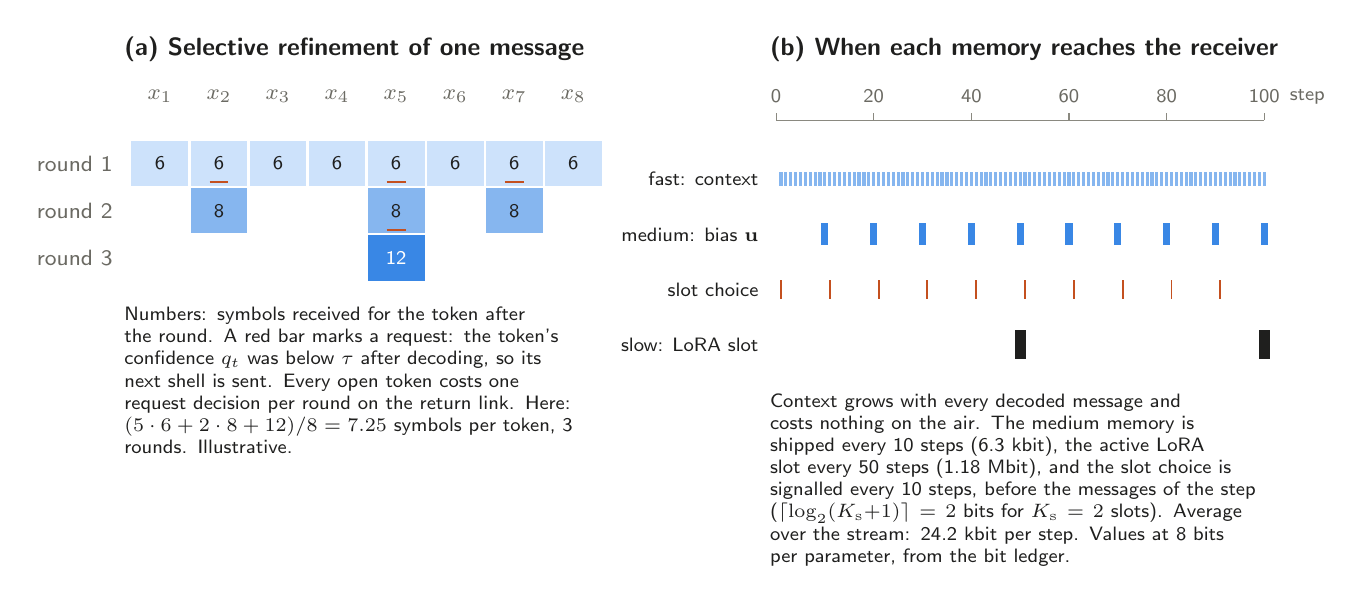
\begin{tikzpicture}[font=\footnotesize, text=ink, >={Stealth[length=2mm,width=1.5mm]}]
% ================= (a) refinement rounds for one message (schematic)
\def\cw{7.5mm}\def\ch{6mm}
\node[anchor=west, font=\small\bfseries] at (-0.2,1.15) {(a) Selective refinement of one message};
% token labels
\foreach \t in {1,...,8} { \node[text=muted] at ({(\t-0.5)*\cw}, 0.55) {$x_{\t}$}; }
% rows: round r, cumulative symbols per token
% round 1: 6 symbols for every token
\foreach \t in {1,...,8} { \fill[s1, draw=white, line width=0.8pt] ({(\t-1)*\cw},0) rectangle ++(\cw,-\ch); \node at ({(\t-0.5)*\cw},{-0.5*\ch}) {\scriptsize 6}; }
% round 2: requested tokens 2,5,7 get +2
\foreach \t in {2,5,7} { \fill[s2, draw=white, line width=0.8pt] ({(\t-1)*\cw},{-\ch}) rectangle ++(\cw,-\ch); \node at ({(\t-0.5)*\cw},{-1.5*\ch}) {\scriptsize 8}; }
% round 3: token 5 gets +4
\foreach \t in {5} { \fill[s3, draw=white, line width=0.8pt] ({(\t-1)*\cw},{-2*\ch}) rectangle ++(\cw,-\ch); \node[text=white] at ({(\t-0.5)*\cw},{-2.5*\ch}) {\scriptsize 12}; }
% request marks (after rounds 1 and 2)
\foreach \t in {2,5,7} { \draw[req, line width=0.7pt] ({(\t-0.5)*\cw-1.2mm},{-\ch+0.6mm}) -- ++(2.4mm,0); }
\draw[req, line width=0.7pt] ({4.5*\cw-1.2mm},{-2*\ch+0.6mm}) -- ++(2.4mm,0);
% row labels
\node[anchor=east, text=muted] at (-1mm,{-0.5*\ch}) {round 1};
\node[anchor=east, text=muted] at (-1mm,{-1.5*\ch}) {round 2};
\node[anchor=east, text=muted] at (-1mm,{-2.5*\ch}) {round 3};
% explanation
\node[anchor=north west, align=left, text width=62mm, font=\scriptsize, execute at begin node={\hyphenpenalty=10000 \exhyphenpenalty=10000 }] at (-0.2,{-3*\ch-2mm}) {Numbers: symbols received for the token after the round. A red bar marks a request: the token's confidence $q_t$ was below $\tau$ after decoding, so its next shell is sent. Every open token costs one request decision per round on the return link. Here: \mbox{$(5\cdot 6+2\cdot 8+12)/8=7.25$} symbols per token, 3 rounds. Illustrative.};

% ================= (b) synchronisation schedule of the memories
\begin{scope}[xshift=82mm]
\node[anchor=west, font=\small\bfseries] at (-0.2,1.15) {(b) When each memory reaches the receiver};
\def\sx{0.62mm}
\draw[line] (0,2.5mm) -- ({100*\sx},2.5mm);
\foreach \x in {0,20,...,100} { \draw[line] ({\x*\sx},2.5mm) -- ++(0,0.9mm); \node[text=muted, font=\scriptsize] at ({\x*\sx},5.5mm) {\x}; }
\node[anchor=west, text=muted, font=\scriptsize] at ({100*\sx+2mm},5.5mm) {step};
% rows
\def\rowA{-5mm}\def\rowB{-12mm}\def\rowC{-19mm}\def\rowD{-26mm}
\node[anchor=east, align=right, font=\scriptsize] at (-1mm,\rowA) {fast: context};
\node[anchor=east, align=right, font=\scriptsize] at (-1mm,\rowB) {medium: bias $\mathbf{u}$};
\node[anchor=east, align=right, font=\scriptsize] at (-1mm,\rowC) {slot choice};
\node[anchor=east, align=right, font=\scriptsize] at (-1mm,\rowD) {slow: LoRA slot};
\foreach \x in {1,...,100} { \fill[s2] ({\x*\sx-0.2mm},{\rowA-0.9mm}) rectangle ++(0.4mm,1.8mm); }
\foreach \x in {10,20,...,100} { \fill[s3] ({\x*\sx-0.45mm},{\rowB-1.4mm}) rectangle ++(0.9mm,2.8mm); }
\foreach \x in {1,11,...,91} { \draw[req, line width=0.7pt] ({\x*\sx},{\rowC-1.2mm}) -- ++(0,2.4mm); }
\foreach \x in {50,100} { \fill[ink] ({\x*\sx-0.7mm},{\rowD-1.8mm}) rectangle ++(1.4mm,3.6mm); }
\node[anchor=north west, align=left, text width=62mm, font=\scriptsize, execute at begin node={\hyphenpenalty=10000 \exhyphenpenalty=10000 }] at (-2mm,{\rowD-5mm}) {Context grows with every decoded message and costs nothing on the air. The medium memory is shipped every 10 steps (6.3~kbit), the active LoRA slot every 50 steps (1.18~Mbit), and the slot choice is signalled every 10 steps, before the messages of the step ($\lceil\log_2(K_\mathrm{s}{+}1)\rceil=2$ bits for $K_\mathrm{s}=2$ slots). Average over the stream: 24.2~kbit per step. Values at 8 bits per parameter, from the bit ledger.};
\end{scope}
\end{tikzpicture}
\end{document}
